\documentclass[12pt]{article}

\usepackage{verbatim}
\usepackage{listings}
\usepackage{color}
\usepackage{graphicx}
\usepackage{amsmath}


%%
\title{Biot Savart Law}

\author{Fabien Le Mentec\\
\small \texttt{texane@gmail.com}
}

\date{}

\begin{document}
\maketitle

%%
\newpage
\begin{abstract}
Notes on the Biot Savart law.
\end{abstract}

%%
\newpage
\section{The Biot Savart Law}

\subsection{B field produced by a current}
\paragraph{} A current $I$ produces a magnetic field $\vec{B}$. $\vec{B}$ has the following characteristics:
\begin{itemize}
  \item its magnitude is \textbf{inversely proportionnal to the square of the distance} between the
    wire and the observation point,
  \item it is \textbf{tangential} to the current direction.
\end{itemize}

\subsection{Biot Savart law}
\paragraph{} The Biot Savart law is used to compute the magnetic field (\textit{Bfield}) produced by
\textbf{steady} a current in a \textbf{straight} portion of a wire. Complex current paths are computed
by decomposing in \textbf{small wire portions}, called $\vec{dl}$.
\begin{center}
  \framebox[3in][c]{$ B = \frac{\mu_{0} \times I}{4 \times \Pi} \int \frac{dl \times \hat{r} }{r^{2}} $}
\end{center}
where:
\begin{itemize}
\item $\mu_{0}$ the vacuum permeability,
\item $I$ the current intensity,
\item $\vec{dl}$ the current direction vector,
\item $\hat{r}$ a unit vector in the direction of $r$,
\item $r$ the distance between the location of $dl$ and the measurement point.
\end{itemize}
This forumla clearly shows:
\begin{itemize}
  \item the magnitude varies with the square of the distance,
  \item the B field is normal to the plan (ie. because of the cross product).
\end{itemize}

\begin{center}
  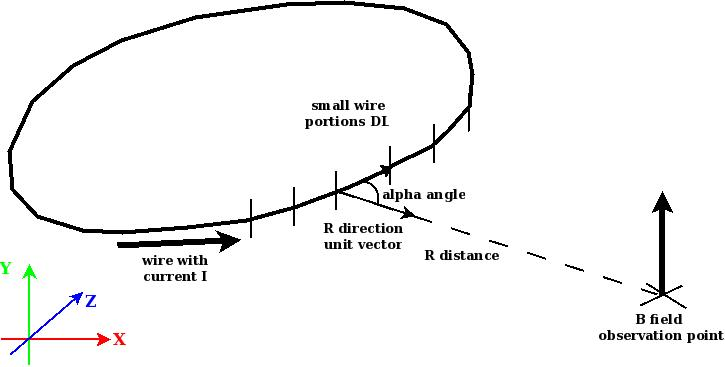
\includegraphics[keepaspectratio=true, width=1.\textwidth]{../dia/bfield_integration/main.jpg}
\end{center}

\subsection{Solenoid B field approximation}
\paragraph{} At the \textbf{center} of \textbf{long} a solenoid (that is, whose length is greater than
diameter), the B field can be approximated with the formula:
\begin{center}
  \framebox[3in][c]{$B = \mu \times n \times l $}
\end{center}
where:
\begin{itemize}
  \item $\mu$ the medium permeability,
  \item $n$ the turn density,
  \item $l$ the solenoid length.
\end{itemize}

\begin{center}
  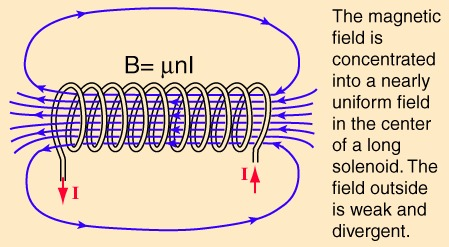
\includegraphics[keepaspectratio=true, width=1.\textwidth]{../pics/solenoid_bfield_approx.jpg}
\end{center}


%%
\newpage
\section{Vector cross product}
\begin{center}
  \includegraphics[keepaspectratio=true, width=65mm]{../pics/cross_product.jpg}\\
\end{center}
\paragraph{} The cross product of 2 vectors $\vec{A}$ and $\vec{B}$ is \textbf{another vector}
$\vec{A} \times \vec{B}$. $\vec{A} \times \vec{B}$:
\begin{itemize}
  \item has the same \textbf{magnitude} as the diagonal of the parallelogram formed by $\vec{A}$
    and $\vec{B}$,
  \item is \textbf{normal} to the plan formed by $\vec{A}$ and $\vec{B}$.
\end{itemize}
Mathematically:
\begin{center}
  \framebox[3in][c]{$ \vec{A} \times \vec{B} = sin(\alpha) \times |A| \times |B| \times \hat{n} $}
\end{center}
where:
\begin{itemize}
\item $\alpha$ is the angle between $\vec{A}$ and $\vec{B}$,
\item $\hat{n}$ is a vector normal to than plan containing $\vec{A}$ and $\vec{B}$.
\end{itemize}

%%
\newpage
\section{References}
\begin{itemize}
\item http://academicearth.org/lectures/biot-savart-law-gauss-law-for-magnetic-fields
\item http://en.wikipedia.org/wiki/Biot\%E2\%80\%93Savart\_law
\item http://dev.physicslab.org/Document.aspx?doctype=3\&filename=Magnetism\_BiotSavartLaw.xml
\end{itemize}


\end{document}
